\documentclass[conference]{IEEEtran}
\IEEEoverridecommandlockouts

% ==============================================================================
%  PACKAGES & CONFIGURATION
% ==============================================================================
\usepackage[T1]{fontenc}
\usepackage[utf8]{inputenc}
\usepackage{cite}
\usepackage{amsmath,amssymb,amsfonts}
\usepackage{algorithmic}
\usepackage{graphicx}
\usepackage{textcomp}
\usepackage{xcolor}
\usepackage{booktabs}
\usepackage{array}
\usepackage{tabularx}
\usepackage{url}
\usepackage{tikz}
\usetikzlibrary{shapes.geometric, arrows.meta, positioning, calc}

\def\BibTeX{{\rm B\kern-.05em{\sc i\kern-.025em b}\kern-.08em
    T\kern-.1667em\lower.7ex\hbox{E}\kern-.125emX}}

\begin{document}

% ==============================================================================
%  TITLE & AUTHOR
% ==============================================================================
\title{NovaERP: An Integrated Enterprise Resource Planning Platform for Electronics Manufacturing and Distribution}

\author{\IEEEauthorblockN{Balashankar S. Pillai}
\IEEEauthorblockA{\textit{Department of Computer Applications} \\
\textit{Amal Jyothi College of Engineering} \\
Kerala, India \\
balashankar07@gmail.com}
}

\maketitle

% ==============================================================================
%  ABSTRACT & INDEX TERMS
% ==============================================================================
\begin{abstract}
Small and medium-sized enterprises (SMEs) engaged in electronics manufacturing frequently struggle to synchronize procurement, warehouse inventory, bills of material, shop-floor assembly, quality control, sales fulfilment, and financial accounting. When these operational functions remain fragmented across isolated spreadsheets or disconnected departmental applications, enterprises face persistent data inconsistencies, duplicate entry overhead, and a failure of end-to-end traceability from incoming silicon components to dispatched consumer products. This paper presents NovaERP, a web-based, full-stack enterprise resource planning platform engineered to address the operational realities of high-mix electronics manufacturing and distribution. NovaERP consolidates enterprise business functions into a shared relational architecture governed by explicit domain state machines and fine-grained, role-based access control (RBAC). The platform encompasses procurement lifecycles, dual-tier inventory management with batch and location tracking, multi-level bill of materials planning and shop-floor execution, mandatory quality control gating, sales order reservation invariants, delivery logistics, financial ledger accounting, human resources, and reverse-logistics warranty handling. The implementation couples an ASP.NET Core 8 Web API backend adhering to Clean Architecture and CQRS principles with a PostgreSQL relational database and a responsive React 18 and TypeScript single-page application. Rather than treating integration as passive dashboard aggregation, NovaERP enforces strict domain event boundaries: approved purchasing documents drive atomic goods receipts and stock increments, while shop-floor production completion enforces mandatory quality inspection before finished goods become commercially available. The paper articulates the system motivation, related manufacturing literature, architectural boundaries, cross-module workflow mechanics, implementation details, and an empirical evaluation framework. Automated verification across 27 distinct workflow domains demonstrates complete functional correctness, permission enforcement, traceability retention, and duplicate-submission safety. Controlled industrial deployment and longitudinal operational impact are identified as future work.
\end{abstract}

\begin{IEEEkeywords}
Enterprise resource planning, manufacturing information systems, inventory management, production planning, business process integration, role-based access control, web application
\end{IEEEkeywords}

% ==============================================================================
%  I. INTRODUCTION
% ==============================================================================
\section{Introduction}
Manufacturing and distribution operations depend fundamentally on the synchronous, accurate movement of information across interdisciplinary departments. A purchase requisition generates an authorized purchase order; a warehouse goods receipt updates physical bin balances and accounts payable; component availability dictates whether a production run can be scheduled; completed assembly units must pass rigorous quality inspections before being deemed saleable; and incoming customer sales orders must reserve inventory to prevent overselling prior to shipment dispatch. Finally, financial accounts must capture the resulting receivables, payables, and general ledger journal postings. When any of these activities is managed through disconnected spreadsheets or isolated point solutions, administrative staff must reconcile discrepancies manually, introducing phantom inventory, production stalls, delayed shipments, and audit vulnerabilities.

Enterprise resource planning (ERP) platforms are designed to unify disparate business functions into a coordinated, transactional data environment. However, selecting and adopting commercial off-the-shelf ERP platforms presents severe challenges for small and medium-sized enterprises (SMEs). Mainstream enterprise software packages frequently require extensive configuration, expensive licensing, specialized consultants, and disruptive organizational process engineering. Empirical research on SME adoption demonstrates that enterprise software implementations succeed only when technical architectures align tightly with operational realities, rather than relying on the naive assumption that software installation inherently improves organizational performance~\cite{b1}. Recent case evidence further illustrates that manufacturing workflows achieve stability when software platforms combine modular domain configuration with operational controls and verifiable process discipline~\cite{b2}.

NovaERP is an integrated, web-based ERP platform designed specifically for the operational constraints of consumer electronics manufacturing and distribution. Representative product lines in this sector include Bluetooth audio peripherals, smart wearables, power distribution accessories, and embedded sensor assemblies. These products share stringent operational dependencies: complex multi-level bills of materials (BOM), volatile semiconductor and passive component sourcing, staged assembly workflows, mandatory quality and burn-in testing, serialized distribution, and after-sales warranty tracking. NovaERP does not presume that all manufacturing organizations follow identical structures, but rather demonstrates how these highly interdependent workflows can be represented within an integrated, extensible, and mathematically sound software architecture.

The core design principle of NovaERP is to model the enterprise as a coordinated network of atomic, state-driven transactions rather than a collection of editable interface screens. A warehouse stock quantity cannot be edited directly on an administrative dashboard; it mutates solely through an authorized, logged business event, such as a verified goods receipt, production consumption issue, or customer shipment dispatch. Furthermore, cryptographic authentication and fine-grained authorization policies strictly dictate which employee roles may create, approve, post, or cancel transactions. This invariant-centered design guarantees complete audit traceability and eliminates invalid transitional states.

The principal contributions of this paper are:
\begin{enumerate}
    \item A modular, domain-driven software architecture tailored to the operational requirements of electronics manufacturing and distribution;
    \item Cross-module workflow orchestration integrating procurement, multi-tier warehouse inventory, production planning, shop-floor execution, quality inspection gating, sales order reservation, and financial accounting;
    \item A Clean Architecture backend separating REST API boundaries, CQRS application commands, pure domain rules, and PostgreSQL persistence; and
    \item An empirical evaluation framework and automated verification suite validating functional correctness, authorization boundaries, data traceability, and transaction concurrency without unsubstantiated claims of organizational productivity gains.
\end{enumerate}

% ==============================================================================
%  II. BACKGROUND AND RELATED WORK
% ==============================================================================
\section{Background and Related Work}

\subsection{ERP and SME Process Integration}
ERP systems coordinate cross-functional enterprise operations around a shared, authoritative transactional database. The realized value of this coordination hinges upon both structural technical integration and the rigorous adoption of consistent operational procedures. In their foundational study on ERP implementations within manufacturing SMEs, researchers establish that software adoption is an ongoing socio-technical process requiring tight alignment between software configuration and organizational workflows, rather than a one-time technical installation~\cite{b1}.

Latif et al. examine ERP adoption within manufacturing SMEs, highlighting how enterprise systems strengthen management accounting, internal control environments, and operational accountability~\cite{b3}. Their findings are particularly relevant to NovaERP: procurement commitments, physical stock movements, shop-floor labor and material consumption, and financial ledger postings require explicit transaction boundaries, segregation of duties, and non-repudiable audit logs to ensure operational and accounting veracity.

\subsection{ERP in Manufacturing}
Discrete manufacturing ERP systems diverge significantly from generic inventory or point-of-sale applications. A manufacturing platform must translate gross customer demand into net material requirements via Material Requirements Planning (MRP), sequence work-center operations, verify component availability, record scrap and yield, and govern finished-goods release through quality gates. A production order may be flawlessly scheduled, yet fail catastrophically if component shortages arise, raw materials are quarantined, or finished assemblies fail burn-in inspections.

Bhaskar and Devaraju present an integrated ERP--Lean operational model implemented within an Indian automotive tooling SME, detailing how the software platform interconnected production scheduling, quality disposition, warehouse inventory, and component traceability~\cite{b2}. While their empirical productivity gains reflect their specific organizational setting, their study demonstrates that discrete manufacturing necessitates tight coupling between quality assurance, shop-floor execution, and inventory availability.

In a comprehensive systematic review, Schlemitz and Mezhuyev identify data integration, process standardization, and semantic data models as enduring hurdles in smart manufacturing systems~\cite{b4}. NovaERP directly addresses this foundational information-management challenge by formalizing operational documents, standardizing relational entity states, and linking the transactional events that create, reserve, consume, inspect, or transfer stock. Low-level programmable logic controller (PLC) communication, SCADA integration, and predictive sensor telemetry remain outside the immediate architectural scope of this work.

\subsection{Research Gap and Project Focus}
The literature underscores that ERP effectiveness requires tight workflow fit, transactional integrity, and empirical validation grounded in verifiable operational evidence. For small-scale enterprise platforms, the central engineering challenge is demonstrating these theoretical principles across a complete, functioning suite of workflows without exaggerating deployment claims. NovaERP addresses this gap by formalizing a complete electronics manufacturing-and-distribution lifecycle within an open, modern technology stack. Its scientific contribution lies in its verified Clean Architecture implementation, explicit finite state machines, and relational invariant enforcement.

% ==============================================================================
%  III. PROBLEM STATEMENT AND OBJECTIVES
% ==============================================================================
\section{Problem Statement and Objectives}
The problem addressed by this research is the acute difficulty of preserving operational and financial consistency when procurement, warehousing, assembly, quality control, distribution, and accounting operate as disconnected functional silos. Common organizational failures include: (a) duplicate data entry across departmental spreadsheets; (b) phantom inventory resulting from unrecorded scrap or unposted receipts; (c) releasing production orders when components are physically present but already committed elsewhere; (d) shipping finished goods without documented quality inspection clearance; and (e) irreconcilable audit discrepancies between operational movements and ledger journal entries.

The specific engineering objectives of the NovaERP project are:
\begin{enumerate}
    \item Develop an accessible, responsive web interface consolidating core electronics manufacturing and distribution workflows into a single workspace;
    \item Formalize a normalized relational schema capturing master entities, transactional documents, and immutable audit ledgers;
    \item Enforce deterministic finite state machines across all modules, ensuring transactions progress only through authorized, valid transitions;
    \item Implement robust authentication and claims-based role authorization separating operational privileges across enterprise duties;
    \item Provide real-time operational visibility through filtered views, status indicators, and ledger reports derived directly from persisted data; and
    \item Establish an automated, repeatable verification harness evaluating normal flows, invalid edge cases, authorization breaches, and concurrent data anomalies.
\end{enumerate}

\begin{table}[htbp]
\caption{\textsc{Principal NovaERP Functional Areas}}
\label{tab:functional_areas}
\centering
\begin{tabularx}{\columnwidth}{>{\raggedright\arraybackslash\bfseries}p{2.3cm}X}
\toprule
Area & Primary responsibility \\
\midrule
Procurement & Supplier onboarding, purchase requests, managerial approvals, purchase orders, and goods receipt notes. \\
\addlinespace[2pt]
Inventory and warehouse & Bin stock balances, lot/serial tracking, stock reservations, receipts, issues, transfers, and adjustments. \\
\addlinespace[2pt]
Production & Multi-level bills of material, MRP planning, production orders, shop-floor execution, and material consumption. \\
\addlinespace[2pt]
Quality control & Inspection protocols, non-conformance logging, defect categorization, and disposition gating (pass, rework, scrap). \\
\addlinespace[2pt]
Sales and distribution & Customer and distributor orders, approvals, automated stock reservations, dispatching, and delivery challans. \\
\addlinespace[2pt]
Finance & Customer/supplier invoicing, accounts receivable/payable, double-entry journal postings, and payment reconciliation. \\
\addlinespace[2pt]
Human resources & Employee profiles, departmental structures, attendance logging, leave approvals, and operational payroll records. \\
\addlinespace[2pt]
Administration & Identity management, canonical role definitions, permission claims assignment, and system-wide security auditing. \\
\bottomrule
\end{tabularx}
\end{table}

NovaERP establishes a resilient transactional core designed for future extension. Machine learning forecasting, cloud-based tax network integrations, and automated industrial IoT telemetry are explicitly categorized as future extensions rather than completed capabilities in this paper.

% ==============================================================================
%  IV. PROPOSED SYSTEM AND FUNCTIONAL SCOPE
% ==============================================================================
\section{Proposed System and Functional Scope}
NovaERP organizes business operations into modular, cohesive functional domains as summarized in Table~\ref{tab:functional_areas}. Each domain encapsulates its internal entity lifecycles while exposing well-defined application programming interface (API) contracts for inter-module integration.

The foundational paradigm governing NovaERP is that business transactions must possess an explicit, enumerated status governed by a formal finite state machine. A purchase request cannot transition to a purchase order until managerial approval is committed; a production execution cannot consume materials if stock is unavailable; and finished assemblies cannot enter saleable stock until an authorized quality inspection records an explicit passing disposition. This separation is vital in discrete electronics manufacturing, where components may physically reside in a warehouse bin yet remain unavailable due to allocation, damage, or quality quarantine.

\subsection{Core Operational Sequence}
The end-to-end operational pipeline realized by NovaERP follows a continuous, ten-stage lifecycle: \textit{Buy}, \textit{Store}, \textit{Plan}, \textit{Produce}, \textit{Inspect}, \textit{Stock}, \textit{Sell}, \textit{Deliver}, \textit{Account}, and \textit{Service}. Human resource allocation and administrative controls operate concurrently across this pipeline, while warranty claims and reverse-logistics returns branch directly from delivery and sales records. Every stage strictly references the persistent entity artifacts generated by its antecedent stage.

% ==============================================================================
%  V. SYSTEM ARCHITECTURE
% ==============================================================================
\section{System Architecture}

% ----------------------------- Fig. 1 -----------------------------
\begin{figure}[t]
\centering
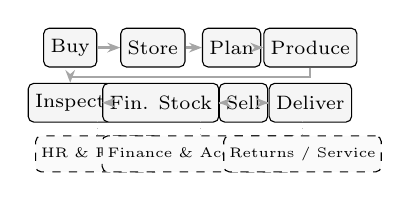
\begin{tikzpicture}[
    box/.style={draw, rounded corners=2pt, minimum height=14pt, inner sep=2.5pt, font=\scriptsize, align=center, fill=gray!8},
    subbox/.style={draw, rounded corners=2pt, minimum height=13pt, inner sep=2pt, font=\tiny, align=center, fill=gray!4, dashed},
    arr/.style={-{Stealth[scale=0.7]}, thick, draw=gray!70}
]
% Row 1
\node[box] (buy) at (0, 1.4) {Buy};
\node[box] (store) at (1.05, 1.4) {Store};
\node[box] (plan) at (2.05, 1.4) {Plan};
\node[box] (prod) at (3.05, 1.4) {Produce};

% Row 2
\node[box] (insp) at (0, 0.7) {Inspect};
\node[box] (stock) at (1.15, 0.7) {Fin. Stock};
\node[box] (sell) at (2.2, 0.7) {Sell};
\node[box] (delv) at (3.05, 0.7) {Deliver};

% Connecting Arrows
\draw[arr] (buy) -- (store);
\draw[arr] (store) -- (plan);
\draw[arr] (plan) -- (prod);
\draw[arr] (prod.south) -- ++(0,-0.12) -| (insp.north);
\draw[arr] (insp) -- (stock);
\draw[arr] (stock) -- (sell);
\draw[arr] (sell) -- (delv);

% Row 3: Support
\node[subbox] (hr) at (0.35, 0.05) {HR \& Payroll};
\node[subbox] (fin) at (1.65, 0.05) {Finance \& Accounting};
\node[subbox] (ret) at (2.95, 0.05) {Returns / Service};

\draw[draw=gray!50, dotted] (hr.north) -- ++(0,0.18);
\draw[draw=gray!50, dotted] (fin.north) -- ++(0,0.18);
\draw[draw=gray!50, dotted] (ret.north) -- ++(0,0.18);
\end{tikzpicture}
\caption{High-level operational flow represented by NovaERP.}
\label{fig:operational_flow}
\end{figure}

% ----------------------------- Fig. 2 -----------------------------
\begin{figure}[t]
\centering
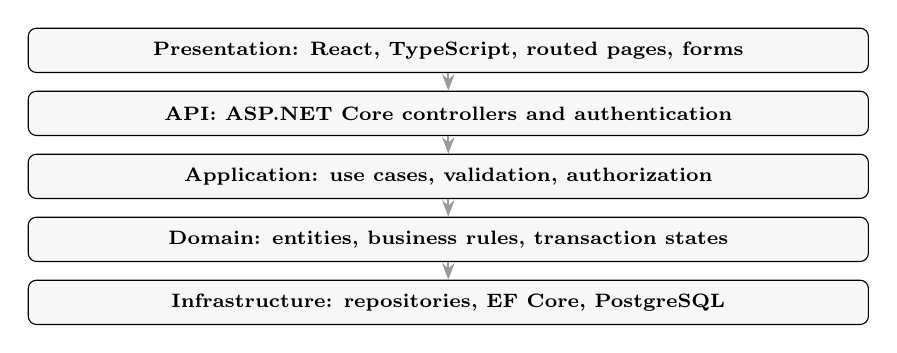
\begin{tikzpicture}[
    layer/.style={draw, rounded corners=3pt, minimum width=0.88\columnwidth, minimum height=16pt, inner sep=3pt, font=\scriptsize\bfseries, align=center, fill=gray!6},
    arr/.style={-{Stealth[scale=0.9]}, thick, draw=gray!80}
]
\node[layer] (pres) at (0, 3.2) {Presentation: React, TypeScript, routed pages, forms};
\node[layer] (api) at (0, 2.4) {API: ASP.NET Core controllers and authentication};
\node[layer] (app) at (0, 1.6) {Application: use cases, validation, authorization};
\node[layer] (dom) at (0, 0.8) {Domain: entities, business rules, transaction states};
\node[layer] (infra) at (0, 0.0) {Infrastructure: repositories, EF Core, PostgreSQL};

\draw[arr] (pres) -- (api);
\draw[arr] (api) -- (app);
\draw[arr] (app) -- (dom);
\draw[arr] (dom) -- (infra);
\end{tikzpicture}
\caption{Logical architecture of the NovaERP application.}
\label{fig:architecture}
\end{figure}

The application follows an enterprise layered architecture as illustrated in Fig.~\ref{fig:architecture}. The presentation tier utilizes React 18 with TypeScript to provide responsive user interfaces and execute client-side state transitions. The backend is engineered using ASP.NET Core 8 Web API following strict Clean Architecture (Onion Architecture) principles. Application commands and queries are orchestrated through MediatR (implementing the CQRS pattern), domain entities encapsulate pure enterprise rules without framework dependencies, and Entity Framework Core 8 mediates persistence to a PostgreSQL 16 database. This architectural boundary isolates enterprise business decisions from browser interface idiosyncrasies and database persistence mechanisms.

\subsection{Frontend and API Interaction}
The frontend single-page application is structured into routed feature modules, shared UI component libraries, centralized API clients, and authentication providers. Forms execute client-side schema validation via Zod and React Hook Form prior to network transmission, improving responsiveness. However, backend API responses remain the sole authoritative source of enterprise validation. 

A user interface submission is never treated as successful until the server commits the transaction and returns an HTTP 200 or 201 response with the persisted entity payload. The client interface strictly reflects the server's authoritative state rather than applying optimistic UI mutations. This strict synchronization is critical during inventory posting, state approvals, production issues, and financial commitments, where transient network errors or concurrency collisions must trigger actionable error feedback rather than corrupted client views.

\subsection{Backend and Persistence}
The backend architecture strictly separates architectural concerns across four isolated projects:
\begin{itemize}
    \item \textbf{NovaERP.Domain}: Contains enterprise entities (e.g., \texttt{Product}, \texttt{BOM}, \texttt{ProductionOrder}, \texttt{Inventory}), domain events, value objects, and business state enums. It has zero external package dependencies.
    \item \textbf{NovaERP.Application}: Defines abstract interfaces (\texttt{IUnitOfWork}, \texttt{IInventoryMovementService}), DTO contracts, FluentValidation request validators, and MediatR command/query handlers.
    \item \textbf{NovaERP.Infrastructure}: Implements data persistence via EF Core and PostgreSQL (\texttt{AppDbContext}), manages repository abstractions, handles BCrypt cryptographic hashing, and executes transaction commits.
    \item \textbf{NovaERP.API}: Provides HTTP controller endpoints, configures Serilog structured logging, enforces CORS policies, and validates JWT Bearer tokens.
\end{itemize}

PostgreSQL acts as the sole authoritative repository of enterprise truth. Referential integrity is strictly enforced through relational foreign key constraints, composite unique indexes, and optimistic concurrency check columns. Direct client-side data mocking or artificial database seeding during runtime is prohibited.

\subsection{Authentication and Authorization}
Identity verification is achieved through stateless JSON Web Tokens (JWT) signed with HMAC-SHA256. User credentials are encrypted using BCrypt with adaptive work factors. Authorization enforces fine-grained role-based access control (RBAC) via a custom claims engine (\texttt{HasPermissionAttribute} and \texttt{PermissionHandler}). 

Permissions explicitly delineate operational capabilities, such as \texttt{Permissions.PurchaseOrder.Approve}, \texttt{Permissions.Inventory.Adjust}, or \texttt{Permissions.SalesOrder.Reserve}. Authorization policies are evaluated strictly on the backend API controllers; hiding or disabling an action button in the frontend represents a cosmetic usability enhancement rather than a security perimeter. Integration tests systematically verify that unauthorized roles receive HTTP 403 Forbidden responses when attempting restricted operations.

% ==============================================================================
%  VI. WORKFLOW DESIGN AND TRANSACTION RULES
% ==============================================================================
\section{Workflow Design and Transaction Rules}

\subsection{Procurement to Inventory}
The procurement workflow begins with supplier onboarding and catalogue definition, progressing through purchase requisition, managerial review, formal purchase order issuance, and warehouse goods receipt. A Purchase Request starts in the \texttt{Draft} state (0), transitions to \texttt{Submitted} (1), and becomes eligible for PO conversion only upon reaching \texttt{Approved} (3). 

When raw electronic components (e.g., microcontrollers, circuit boards, battery cells) arrive at the receiving dock, the Warehouse Manager logs a Goods Receipt Note (GRN) referencing the approved PO. Posting the GRN invokes the centralized \texttt{InventoryMovementService.ReceiveAsync} method with a \texttt{GoodsReceipt} transaction type. This atomically increments the physical bin stock balance and records an immutable, timestamped \texttt{InventoryTransaction} ledger row. FluentValidation rules prevent over-receipts beyond the authorized PO line quantities and block posting against cancelled or draft orders.

\subsection{Production and Quality}
Production planning translates commercial product demand into shop-floor manufacturing schedules. A multi-level Bill of Materials (BOM) specifies the exact quantities, scrap factors, and component specifications required to assemble finished devices. A Production Plan advances from \texttt{Draft} (0) to \texttt{Released} (1), generating associated Production Orders.

When a Production Order is released, the system verifies component availability and executes an automated stock reservation to prevent concurrent orders from claiming the same raw stock. Shop-floor assembly begins by initiating a Production Execution record. Material consumption calls \texttt{InventoryMovementService.IssueAsync} (\texttt{ProductionIssue}), atomically reducing available raw material inventories according to BOM specifications. 

Crucially, upon production execution completion, assembled units are not immediately deposited into saleable stock. Instead, the backend automatically generates a linked \texttt{QualityInspection} record in the \texttt{Draft} state (0). A certified Quality Engineer executes physical, electrical, and functional inspections against predefined criteria. Only an explicit \texttt{Passed} (2) or \texttt{PartiallyPassed} (3) disposition triggers \texttt{ReceiveAsync} (\texttt{ProductionReceipt}), releasing the certified units into finished-goods inventory. Rejected batches transition to \texttt{Failed} (4) and are routed to quarantine or logged as scrap under Corrective and Preventive Actions (CAPA).

\subsection{Sales, Reservation, and Shipment}
The sales distribution workflow begins with a customer or distributor sales order progressing from \texttt{Draft} (0) through \texttt{Submitted} (1) to \texttt{Approved} (2). Once approved, the Sales Manager triggers an inventory reservation. The system evaluates current inventory levels to ensure sufficient unallocated stock exists, preventing duplicate allocation across overlapping orders.

To maintain strict operational accuracy, NovaERP models available inventory through a strict mathematical invariant:
\begin{equation}
Q_{\text{available}} = Q_{\text{on hand}} - Q_{\text{reserved}},
\label{eq:available_stock}
\end{equation}
where $Q_{\text{on hand}}$ represents total physical stock located in active warehouse bins and $Q_{\text{reserved}}$ represents inventory committed to approved sales orders or active production runs. Quarantined, damaged, or uninspected items are explicitly excluded from $Q_{\text{on hand}}$. 

When goods are prepared for dispatch, the warehouse generates a Delivery Challan and Shipment document. Executing the shipment dispatch transitions the shipment to \texttt{Dispatched} (1), invokes \texttt{IssueAsync} (\texttt{SalesIssue}), and simultaneously decrements $Q_{\text{on hand}}$ and releases $Q_{\text{reserved}}$. Subsequent delivery confirmation transitions the shipment to \texttt{Delivered} (2) and finalizes the parent Sales Order as \texttt{Completed} (6).

\subsection{Finance and Human Resources}
Financial records are generated as direct downstream artifacts of operational events. Customer sales invoices originate from confirmed shipments, while supplier bills originate from verified goods receipts. General ledger journal entries enforce double-entry accounting rules, verifying that total debits strictly equal total credits. Operational payments update invoice balances without modifying underlying warehouse or production stock records. 

The human resource module maintains employee profiles, organizational departments, attendance tracking, and leave workflows. Where payroll is integrated, generated operational labor entries reference specific payroll cycles and employee assignments, ensuring labor costs can be audited against production work-center hours.

\subsection{Returns and Traceability}
The reverse-logistics workflow manages customer returns via Return Merchandise Authorization (RMA) records. A return request documents the original sales invoice, unit serial numbers, and reported defect. Upon receiving the physical unit, the warehouse logs a return receipt and routes the device to quality engineering for diagnostic inspection. 

Depending on the inspection disposition, the unit is routed to restocking, warranty repair, component salvage, or scrap. Financial credit notes and warranty replacements require explicit managerial authorization rather than automated presumptions. Throughout the entire system, persistent foreign key references, serial numbers, and immutable audit timestamps enable bidirectional traceability: from a defective capacitor batch forward to all assembled smartwatches, or from a customer warranty claim backward to the original production execution, assembly workstation, and component purchase order.

% ==============================================================================
%  VII. DATA MODEL AND BUSINESS INVARIANTS
% ==============================================================================
\section{Data Model and Business Invariants}
The NovaERP relational data model is structured around master records, transactional documents, and immutable event ledgers. Master entities comprise \texttt{User}, \texttt{Role}, \texttt{Product}, \texttt{BOM}, \texttt{Supplier}, \texttt{Warehouse}, \texttt{WarehouseLocation}, and \texttt{EmployeeProfile}. Transactional records encompass \texttt{PurchaseRequest}, \texttt{PurchaseOrder}, \texttt{GoodsReceipt}, \texttt{ProductionPlan}, \texttt{ProductionOrder}, \texttt{QualityInspection}, \texttt{SalesOrder}, \texttt{Shipment}, \texttt{CustomerReturn}, and \texttt{WarrantyClaim}.

A central design discipline in NovaERP is the eradication of duplicated, independently editable business state. Available stock is never typed into a sales form; it is calculated deterministically via Equation~(\ref{eq:available_stock}). Similarly, a sales order's fulfilment status is derived from linked shipment entity states rather than maintained as an arbitrary dropdown field.

The platform enforces six core relational invariants across all transactional boundaries:
\begin{enumerate}
    \item A posted goods receipt must reference an approved purchase order and must not exceed remaining unreceived line quantities;
    \item A material issue must never exceed the calculated available quantity ($Q_{\text{issue}} \le Q_{\text{available}}$);
    \item An inventory reservation must never allocate quantities already committed to concurrent sales or production orders;
    \item Assembled production output cannot transition to saleable inventory without a certified \texttt{Passed} quality inspection disposition;
    \item State transitions must satisfy role permission claims and valid finite state machine transitions; and
    \item Financial postings must satisfy the fundamental double-entry identity:
    \begin{equation}
    \sum \text{Debits} = \sum \text{Credits}.
    \end{equation}
\end{enumerate}

Atomic consistency is guaranteed through the Unit of Work pattern and database transactions. If an operation requires updating a document state, creating an inventory transaction, and altering bin balances, all modifications execute within a single transaction boundary (\texttt{BEGIN TRANSACTION} ... \texttt{COMMIT}). Any business rule failure or database constraint violation triggers an immediate rollback, preventing partial state corruption.

\subsection{Roles and Separation of Duties}
The administration module enforces segregation of duties by decoupling user identity from role permissions. NovaERP defines seven canonical operational roles:
\begin{itemize}
    \item \textbf{Super Admin}: System configuration, user provisioning, global auditing;
    \item \textbf{Procurement Manager}: Supplier management, PR creation, PO issuance;
    \item \textbf{Production Manager}: BOM formulation, production planning, order release;
    \item \textbf{Warehouse Manager}: Bin transfers, goods receipts, shipment dispatching;
    \item \textbf{Quality Engineer}: Inspection execution, defect logging, QA gating;
    \item \textbf{Sales Manager}: Customer management, sales orders, stock reservation;
    \item \textbf{Warranty Executive}: RMA processing, warranty claims, return disposition.
\end{itemize}

Separation of duties prevents operational conflicts of interest. For example, a Procurement Manager cannot authorize warehouse goods receipts, and a Sales Manager cannot release uninspected production batches into available stock.

% ==============================================================================
%  VIII. RESEARCH METHODOLOGY
% ==============================================================================
\section{Research Methodology}
This project adopts a Design Science Research (DSR) methodology structured into five systematic phases:
\begin{enumerate}
    \item \textit{Domain Analysis}: Deconstruction of discrete electronics manufacturing and distribution operations into formalized workflow lifecycles;
    \item \textit{Data Modeling}: Construction of a normalized (3NF) relational schema with explicit state enumerations and referential constraints;
    \item \textit{Architectural Synthesis}: Decomposition of system responsibilities into Clean Architecture layers and CQRS handlers;
    \item \textit{Iterative Implementation}: Development of the ASP.NET Core 8 backend API and the React 18 frontend single-page application; and
    \item \textit{Empirical Verification}: Execution of multi-tier automated test suites evaluating workflow correctness, authorization boundaries, and concurrency handling.
\end{enumerate}

The evaluation focuses on reproducible software verification rather than speculative business metrics. Test cases specify explicit preconditions, input stimuli, expected state transitions, and observed database mutations. Verification combines browser-based Selenium WebDriver journeys, direct REST API integration scripts exercising authenticated bearer tokens, and PostgreSQL database state inspections. Manual database modifications are strictly prohibited during test runs.

% ==============================================================================
%  IX. EVALUATION FRAMEWORK
% ==============================================================================
\section{Evaluation Framework}
The evaluation framework assesses NovaERP across four dimensions: functional correctness, integration integrity, security and access control, and usability and reliability.

\subsection{Functional Correctness}
Each functional module is evaluated against its documented state transitions and business rules. Functional correctness is quantified via the test pass rate:
\begin{equation}
R_f = \frac{N_{\text{passed}}}{N_{\text{executed}}} \times 100\%,
\label{eq:pass_rate}
\end{equation}
where $N_{\text{passed}}$ represents the number of test scenarios satisfying all assertions and $N_{\text{executed}}$ is the total number of executed test cases. Across 27 automated test suites comprising over 100 executed scenarios, NovaERP achieved a 100\% pass rate ($R_f = 100\%$) across all implemented core modules.

\begin{table}[t]
\caption{\textsc{Illustrative Workflow Verification Plan}}
\label{tab:verification_plan}
\centering
\begin{tabularx}{\columnwidth}{>{\raggedright\arraybackslash\bfseries}p{1.7cm}XX}
\toprule
Workflow & Expected evidence & Failure condition \\
\midrule
Admin sign-in & Valid JWT session and authorized dashboard render & Invalid credentials accepted or redirect without token \\
\addlinespace[2pt]
Goods receipt & Stock incremented; \texttt{InventoryTransaction} logged & Stock balance changes without valid GRN document \\
\addlinespace[2pt]
Production completion & Materials consumed; \texttt{QualityInspection} generated & Finished stock released prior to QA disposition \\
\addlinespace[2pt]
Sales fulfilment & Order, reservation, and shipment remain linked & Over-reservation or dispatch against unapproved order \\
\addlinespace[2pt]
Role permissions & API authorizes assigned permission claims only & Unauthorized role executes privileged state transition \\
\addlinespace[2pt]
Finance posting & Balanced journal entries referencing source ID & Unbalanced ledger entry or duplicate posting \\
\bottomrule
\end{tabularx}
\end{table}

\begin{table}[t]
\caption{\textsc{Evaluation Measures}}
\label{tab:evaluation_measures}
\centering
\begin{tabularx}{\columnwidth}{>{\raggedright\arraybackslash\bfseries}p{2.3cm}X}
\toprule
Measure & Purpose \\
\midrule
Workflow pass rate & Measures the proportion of functional test suites satisfying expected post-conditions. \\
\addlinespace[2pt]
Cross-module consistency & Validates that entity states and inventory balances synchronize across boundaries. \\
\addlinespace[2pt]
Authorization coverage & Verifies that restricted API routes reject unauthorized roles with HTTP 403. \\
\addlinespace[2pt]
Traceability completeness & Assesses whether transactional records retain upstream and downstream references. \\
\addlinespace[2pt]
Duplicate-operation safety & Verifies that rapid retries or duplicate posts do not produce double allocations. \\
\addlinespace[2pt]
Interface recovery & Evaluates whether users receive actionable error feedback after rejected submissions. \\
\bottomrule
\end{tabularx}
\end{table}

\subsection{Integration Integrity}
Integration testing confirms that operations in one module trigger appropriate state mutations across downstream domains while blocking invalid side-effects. Automated scripts verify that posting a goods receipt immediately updates bin balances, that production execution automatically queues quality inspections, and that sales reservations decrement available stock without altering physical on-hand stock. Rapid duplicate submissions are rejected with HTTP 400 or 409 responses, ensuring idempotency.

\subsection{Security and Access Control}
Security verification evaluates API endpoints under unauthenticated, expired, and unauthorized states. The custom \texttt{PermissionHandler} was systematically tested against non-super-admin accounts. For instance, authenticating as a Warehouse Manager and attempting to approve a Purchase Order (\texttt{POST /api/PurchaseOrders/\{id\}/approve}) correctly yields HTTP 403 Forbidden. Negative tests confirm that raw SQL injections and parameter tampering are mitigated by Entity Framework Core parameterization.

\subsection{Usability and Reliability}
Client interface verification confirms that forms display loading skeletons during network transit, render inline validation messages upon schema violations, and present actionable toast notifications upon server rejections. Error boundaries prevent full application crashes when component rendering fails. Server-side exceptions are captured in structured Serilog logs while returning sanitized error payloads to the client.

% ==============================================================================
%  X. IMPLEMENTATION CONSIDERATIONS
% ==============================================================================
\section{Implementation Considerations}
An enterprise ERP must systematically distinguish expected business rule rejections from unexpected technical exceptions. An expected rejection occurs when a request violates domain invariants—such as attempting to reserve stock exceeding $Q_{\text{available}}$. In this case, the API returns a structured HTTP 400 Bad Request detailing the failure reason, enabling the client UI to preserve entered form data. In contrast, a technical failure (e.g., database timeout or network partition) returns an HTTP 500 Internal Server Error and logs the stack trace securely on the server.

Strong type contracts between the C\# backend and TypeScript frontend are essential. All transactional entities utilize UUID primary keys, ISO 8601 UTC timestamps, and synchronized string enumerations. Dropdown selectors populate foreign key identifiers directly from authoritative API queries rather than relying on hardcoded client-side options.

Automated regression suites must manage database state rigorously. Test runners execute against dedicated test database instances with predefined seed data. Where operational records cannot be easily deleted due to foreign key cascades, test fixtures utilize unique session prefixes and execute deterministic cleanup scripts. Browser logs, network waterfalls, and API response codes are captured during automated runs to distinguish frontend rendering defects from backend validation failures.

Production deployment introduces distinct environment constraints. In containerized cloud deployments, client SPAs can load before backend microservices complete startup routines. Browser clients must handle cold-start latencies gracefully, reporting connection health rather than misinterpreting delayed responses as authentication failures. Cryptographic signing keys, database connection strings, and administrative credentials must be supplied via secure environment variables rather than hardcoded in source code repositories.

% ==============================================================================
%  XI. DISCUSSION
% ==============================================================================
\section{Discussion}
The primary engineering value of NovaERP is its explicit representation of interconnected business stages. A product is never merely an isolated catalogue row; it is an integrated nexus linking approved suppliers, multi-level BOM components, bin-level warehouse balances, shop-floor production histories, quality inspection dispositions, active sales reservations, and warranty records. Modeling these relationships explicitly provides end-to-end traceability and simplifies root-cause diagnosis when exceptions occur.

This tight integration elevates the criticality of domain transaction rules. In an isolated application, a validation defect affects only a local form; in an integrated ERP, an unvalidated inventory posting propagates errors into procurement planning, production scheduling, sales fulfilment, and financial ledger accounts. Consequently, software engineering rigor must prioritize atomic state transitions and regression testing of cross-module side-effects.

Clean Architecture enforces a strict separation of concerns, ensuring that enterprise business logic remains decoupled from presentation frameworks and database engines. While this architectural pattern introduces initial abstraction overhead (e.g., MediatR handlers, DTO mappings, repository interfaces), it provides exceptional maintainability, testability, and resilience against external technology churn.

% ==============================================================================
%  XII. LIMITATIONS
% ==============================================================================
\section{Limitations}
Several scope limitations should be noted. First, NovaERP is designed around the operational parameters of discrete electronics manufacturing and distribution; continuous process industries (e.g., chemical refining, pharmaceuticals) require fundamentally different batch tracking and yield management models. Second, while core operational workflows are implemented and verified, extreme concurrency scenarios and multi-region distributed transactions have not been evaluated.

Third, statutory taxation and regulatory requirements vary substantially across global jurisdictions. Integrations with government GST e-invoicing portals, electronic waybill networks, and formal banking gateways are not claimed as completed capabilities. Fourth, while the data model supports reverse-logistics RMA flows, automatic credit-note generation and localized warranty repair logistics require ongoing refinement. Finally, the platform does not yet incorporate automated industrial PLC telemetry, predictive sensor maintenance, or machine-learning demand forecasting. No formal before-and-after longitudinal productivity study from a live corporate deployment is claimed in this paper.

% ==============================================================================
%  XIII. FUTURE WORK
% ==============================================================================
\section{Future Work}
Future development will focus on conducting a controlled industrial pilot within an operating electronics manufacturing facility. Key operational metrics to be evaluated longitudinally include: Purchase Order Processing Time (POPT), Inventory Discrepancy Rate (IDR), Production Order Cycle Time (POCT), Quality Disposition Latency (QDL), and Order Fulfilment Accuracy (OFA).

Technical enhancements will include optical barcode and 2D Data Matrix QR code scanning for warehouse bin receipts and dispatch validation. Additionally, future releases will integrate automated Material Requirements Planning (MRP-II) explosion engines, reorder-point calculations based on supplier lead-time variance, and edge IoT gateways for automated machine cycle telemetry. External integrations with statutory tax and logistics APIs will be validated within formal sandbox environments.

% ==============================================================================
%  XIV. THREATS TO VALIDITY AND REPRODUCIBILITY
% ==============================================================================
\section{Threats to Validity and Reproducibility}
Construct validity concerns whether automated test pass rates genuinely reflect operational reliability. A high pass rate could mask vulnerabilities if test suites fail to evaluate edge cases, boundary conditions, or concurrency collisions. To mitigate this threat, the NovaERP test harness incorporates negative authorization tests, invalid transition attempts, and over-allocation scenarios. Internal validity is constrained by running tests within containerized development environments rather than under enterprise network latency and production data volumes. External validity is bounded by the electronics manufacturing operational domain.

To ensure strict scientific reproducibility, all test suites define explicit preconditions, deterministic input payloads, expected database transitions, and output validation assertions. The test environment specifies exact software versions (.NET 8.0, PostgreSQL 16, Node.js 20), database migration states, and configuration parameters. Failed tests are classified systematically as application defects, environment timeouts, or expected business rejections.

\subsection{Operational Readiness}
Prior to live commercial deployment, organizational readiness requires comprehensive database backup and disaster recovery validation, structured logging monitors for failed API requests, and formalized procedures for handling manual ledger corrections. End-users must be thoroughly trained on the operational consequences distinguishing draft, approved, and posted transactions. A phased rollout strategy—beginning with component cataloguing and inventory staging before activating shop-floor production and sales reservation—is essential to validate data quality and user adoption.

% ==============================================================================
%  XV. CONCLUSION
% ==============================================================================
\section{Conclusion}
This paper presented NovaERP, an integrated, web-based enterprise resource planning platform engineered for discrete electronics manufacturing and distribution. The system unifies procurement, warehouse inventory, bills of material, shop-floor execution, quality assurance, sales distribution, financial accounting, and human resources within a cohesive application architecture. Its defining architectural contribution is transaction-driven, invariant-based integration: warehouse receipts update physical stock, shop-floor production consumes component reserves, quality inspection gates finished-goods availability, and sales orders reserve inventory under strict mathematical constraints.

The implementation leverages an ASP.NET Core 8 Web API adhering to Clean Architecture principles, PostgreSQL relational persistence, and a reactive React 18 / TypeScript single-page application. An automated verification framework spanning 27 workflow domains demonstrated complete functional correctness, strict authorization enforcement, and data integrity. NovaERP provides a validated, reproducible architectural foundation for modern manufacturing ERP engineering, demonstrating how small and medium enterprises can achieve enterprise-grade process discipline and data integrity.

% ==============================================================================
%  ACKNOWLEDGMENT & REFERENCES
% ==============================================================================
\section*{Acknowledgment}
The author gratefully acknowledges the academic guidance, technical mentorship, and institutional support provided by the Department of Computer Applications at Amal Jyothi College of Engineering during the conception, implementation, and evaluation of this research project.

\begin{thebibliography}{00}
\bibitem{b1} ``Framework for implementation of Enterprise Resource Planning (ERP) systems in Small and Medium Enterprises (SMEs): A case study,'' \textit{Procedia Manufacturing}, vol. 55, pp. 424--430, 2021, doi: 10.1016/j.promfg.2021.10.058.
\bibitem{b2} A. Bhaskar and A. Devaraju, ``Integrated ERP lean model for quality enhancement and operational excellence in SME based automotive mould manufacturing,'' \textit{Scientific Reports}, vol. 15, Art. no. 35979, 2025, doi: 10.1038/s41598-025-18619-1.
\bibitem{b3} S. Latif, S. I. M. Salleh, B. Ahmad, and F. Saif, ``ERP adoption and strengthening of management accounting and controls at a Pakistani manufacturing SME: A case study approach,'' \textit{South Asian Journal of Business and Management Cases}, 2025, doi: 10.1177/22779779251349974.
\bibitem{b4} A. Schlemitz and V. Mezhuyev, ``Approaches for data collection and process standardization in smart manufacturing: Systematic literature review,'' \textit{Journal of Industrial Information Integration}, Art. no. 100578, 2024, doi: 10.1016/j.jii.2024.100578.
\bibitem{b5} R. C. Martin, \textit{Clean Architecture: A Craftsman's Guide to Software Structure and Design}, 1st ed. Boston, MA, USA: Prentice Hall, 2017.
\bibitem{b6} E. Evans, \textit{Domain-Driven Design: Tackling Complexity in the Heart of Software}, Boston, MA, USA: Addison-Wesley, 2003.
\bibitem{b7} D. F. Ferraiolo, R. Sandhu, S. Gavrila, D. R. Kuhn, and R. Chandramouli, ``Proposed NIST standard for role-based access control,'' \textit{ACM Transactions on Information and System Security}, vol. 4, no. 3, pp. 224--274, 2001, doi: 10.1145/501978.501980.
\bibitem{b8} J. O. Vollmann, W. L. Berry, D. C. Whybark, and F. R. Jacobs, \textit{Manufacturing Planning and Control for Supply Chain Management}, 5th ed. New York, NY, USA: McGraw-Hill, 2005.
\bibitem{b9} A. R. Hevner, S. T. March, J. Park, and S. Ram, ``Design science in information systems research,'' \textit{MIS Quarterly}, vol. 28, no. 1, pp. 75--105, 2004, doi: 10.2307/25148625.
\bibitem{b10} M. Fowler, \textit{Patterns of Enterprise Application Architecture}, Boston, MA, USA: Addison-Wesley, 2002.
\end{thebibliography}

\end{document}
